
%\addcontentsline{toc}{section}{Introduction} % Ajout dans la table des matières
\section{Résumé} 

Pendant ces quatre mois de stage, notre groupe de recherche travaille avec les employés de \textsc{cmcc} ( China Mobile Communications Corporation ) . Le objectif du sujet est: utilise les technique de Fouille de données, étude les données fournir par CMCC, et trouve les relation entre les données et les défaut du système 4G. Nous avons fait plusieurs tentatives pour trouver les résultats, et on a utilise différents logiciel, j'ai utilisé le R, et mon collègue utilise Mathlab, nous avons utilisé plusieurs algorithme (Clusterring, PCA, Association rules, Ajustement). Mais à la fin,  nous avons trouvé que à cause des défaut dans la système d'acquisition, les données ne sont pas correct, et nous ne pouvons pas trouver le résultat comme prévu. Mais les recherches que nous avons fait peut faites-leur savoir comment utilise les technique de fouille de donnée dans la domaine de télécommunication.

\section{Introduction} 
 
Le 3 avril 1973, M. Mation \textsc{cooper} le directeur général de la division communication de Motorola, à effectuer un appel téléphonique à Joel \textsc{engel}, son rival et néanmoins confrère chez \textsf{Belle Labs}. c'est la premier appel téléphonique en extérieur, L'idée du téléphone portable devient une réalité. 

depuis ce jour, le technique développé très rapidement. dans les 20 dernières années, il y a déjà quatre génération des standards pour la téléphonie mobile, non seulement nous pouvons appeler les autres, les nouvelles technologies et les Smart-phones nous permettons aussi envoyer les message, surfer l'Internet, utiliser le service RTSP(Real Timide Streaming Protocol), et le service VoIP (Voice over Internet Protocole),etc.. les services de communication téléphonique sont devenus un outil très important dans notre vie.
 
 \subsection{Introduction du CMCC}
 
Fondé en 3 Septembre 1997, après le regroupement de opérateur des télécommunications en 2008, \textsc{China Mobile Communications Corporation} (\textsf{CMCC})\ref{Fig.sub.1} est devenu un de trois opérateur des télécommunications en Chine (deux autres sont \textsf{China Unicom Co., Ltd.} et \textsf{China Telecom}). Après plusieurs années de développement, il a construit le plus grand réseau de communications mobiles dans le monde, possède la plus grande base d'utilisateurs dans le monde\ref{Fig.sub.2}. En 2013, CMCC a 767 million utilisateurs, 630,2 billion \textyen \qquad de revenu, 121,7 billions \textyen de revenus net, effectif 197,030.
\begin{figure}[H]
	\flushleft
	\subfigure[Logo de China Mobile]{
		\label{Fig.sub.1}
		
\includegraphics[width=1.8in]{images/China_Mobile_2013.png}}\hfill
	\hspace{1in}
%\flushright
	\subfigure[Reseau télécommunication]{
		\label{Fig.sub.2}
		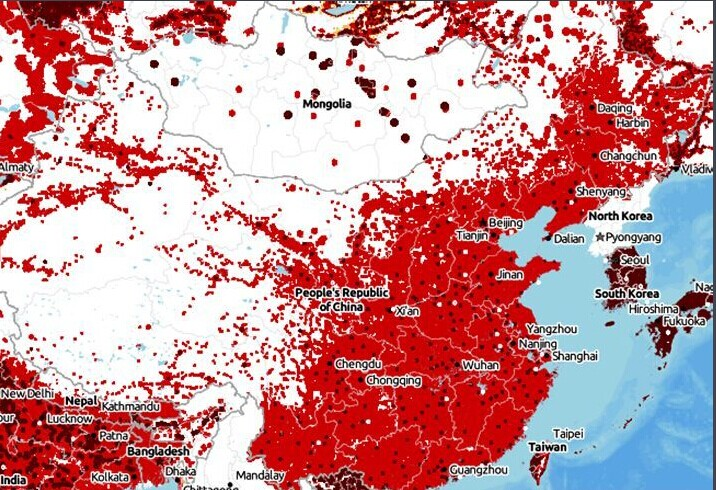
\includegraphics[width=2.0in]{images/reseau.jpg}}
	\caption{CMCC} 
\end{figure}

\subsection{La crise de CMCC}
Mais en même temps, le taux de croissance des nouveaux utilisateur décline de 22,5 \% (2006) à moins de 5\% 2013 \ref{tauxdecroissance}. Et dans la premier 3 mois, l'entreprise une fois considérés comme la plus rentable de Chine, le taux de croissance des revenu net est 0,3\%.

      \begin{figure}[H]
          \centering
          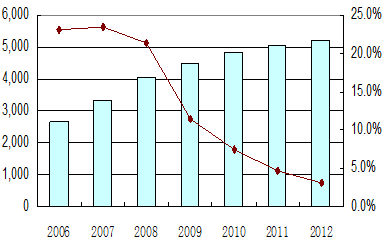
\includegraphics[width=3in]{images/1.png}
          \caption{le taux de croissance est décliner}
          \label{tauxdecroissance}
      \end{figure}
Opérateur des télécommunications Vodafone a fait un étude après il déployé un réseau 3G(\textsf{the third generation of mobile phone mobile communication technology standards}). Comme le réseau 3G permettant des débits (de 2 à 42 Mb/s définis par la dernière génération des réseaux) qui sont bien plus rapides que la génération précédente, par exemple le GSM. Les utilisateur utilisent bien plus souvent le service internet\ref{vodafone1}. Comme ils utilisent plus du service internet, le data ARPU (Average Revenue Per User) augment, mais le voix ARPU décline plus rapide que la montant de data ARPU\ref{vodafone2}. 
 \begin{figure}[H]
 	\flushleft
 	 	\subfigure[Downlink Data Traffic in 2G/3G Network]{
 	 	\label{vodafone1}
 	 	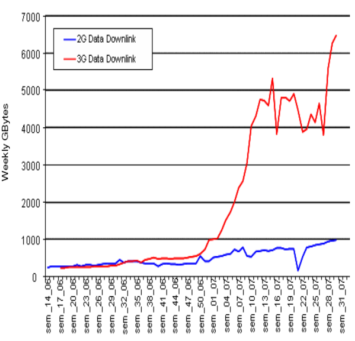
\includegraphics[width=2.0in]{images/4.png}}\hfill
 	\hspace{1in}	 
 	\subfigure[étude de Vodafone]{
 		\label{vodafone2}
 		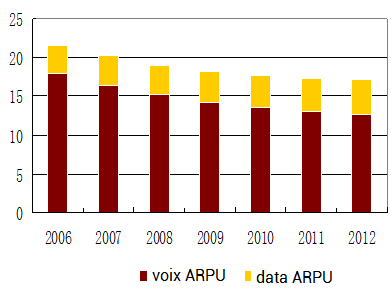
\includegraphics[width=1.8in]{images/2.png}}
 	\caption{Vodafone} 
 \end{figure}
 
Mais l'étude de Orange nous montre que si nous pouvons fournir des nouveaux technologies qui a plus haute débit, les utilisateur utiliseront plus souvent le service data.  \ref{traficparpersonne}
  \begin{figure}[H]
   \centering
   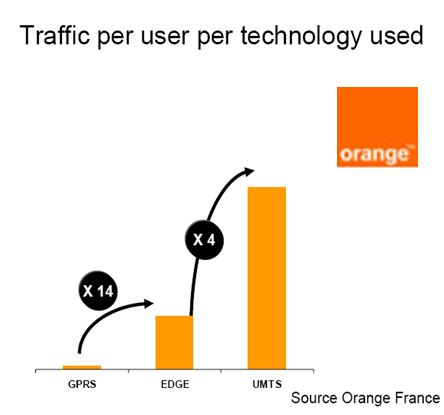
\includegraphics[width=3in]{images/orange.JPG}
   \caption{trafic par personne }
   \label{traficparpersonne}
  \end{figure}
 Des études nous montre nouveaux technologie (comme LTE) peut diminue le prix de revient, qui peut assurer le profit de l'opérateur. Mais déployé les nouveaux matériel coût très cher, en 2009, CMCC dépenser 30 billions \textyen en construit les station pour réseau 3G, et à 2014, CMCC a construit 1,5 million stations, à la fin de cet année, il y aura 1,8 million stations, parmi ces station, il y aura 500 mille stations TD-LTE. En ajoutant des équipement 4G, il peut être mis à niveau un station de 3G à 4G. Donc déployé le réseau 4G n'est pas trop cher, selon l'expérience précédente (de 2G à 3G), les utilisateurs iront utiliser plus le service internet, qui peut assurer le profit de l'entreprise.
      \begin{figure}[H]
          \centering
          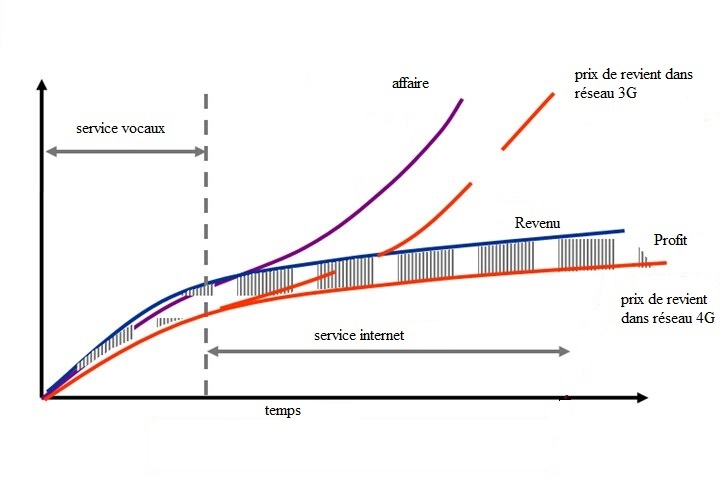
\includegraphics[width=3in]{images/why4G.jpg}
          \caption{4G est plus rentable}
          \label{why4G}
      \end{figure}
  \subsection{L'optimisation du réseau}
A part de la évolution des technologies. Un grand enjeu pour les opérateurs est: l'optimisation du réseau télécommunication. Le réseau de communication mobile est très dynamique, la répartition de la densité du trafic est inégale, fréquence très limité, etc. La configuration du réseau état toujours sous-optimal, et la perception de l'utilisateur n'est pas très bien. Donc tous les opérateurs doivent toujours reconfigurer/optimiser/maintien les paramètre du réseau.
  
Les opérateurs peuvent percevoir les données sur Internet, et utilisent ces informations pour trouver les défauts du système, peut aide l'entreprise optimiser le système.

Mais la optimisation du réseau télécommunication est difficile parce-que: Les technologies d'optimisation de réseau concerné: La technologie de commutation, la technologie sans fil, la configuration et commutation de la fréquence, la signalisation système, l'analyse de trafic, etc. c'est un travail difficile, exiger une meilleure aptitude des employés.  

Actuellement, l'optimisation du réseau dépend principalement à la expérience du personnel. Mais des fois les expériences ne sont pas correct. Par exemple, Si l'entreprise besoin de savoir le congestionné d'un station, il faut envoyer les employé avec des équipement pendant les périodes de pointe, mais on ne sait pas si les résultats sont correct \ref{meseau}.  En outre, souvent un seul type de  donnée ont utilise pour l'analyse et la comparaison pour optimiser les réseau, plutôt que de trouver un solution d'optimisation basées sur toutes les données liées au réseau (telles que les données statistique de trafic, les données d'essai, etc). Et en raison de l'énorme quantité de données, c'est difficile de traite en temps opportun. il est évident que ce méthode est défectueux. Les défauts du système provoque la satisfaction des utilisateurs inférieure, ce qui a conduit à multiplier.
      \begin{figure}[H]
          \centering
          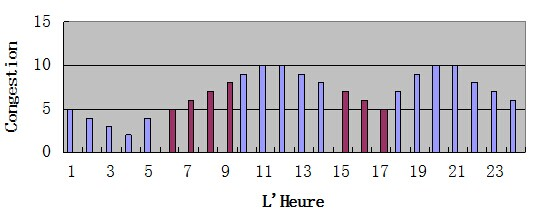
\includegraphics[width=3in]{images/meseau.jpg}
          \caption{Mesure la congestionné d'un station}
          \label{meseau}
      \end{figure}
      
Face à des problèmes complexes, les grands entreprises commence utilise les techniques de Fouille de données. Ce technique peut aide l'entreprise faire les décision plus vite et plus précis.

De ce faire, en Juillet 2013, CMCC a lancé ce projet avec quatre laboratoires dans trois université, ils sont
 \href{http://www.tsinghua.edu.cn/publish/newthuen/index.html}{Tsinghua University}, \href{http://en.sdu.edu.cn/}{Shandong University} et \href{http://www.oice.uestc.edu.cn/en/}{University of Electronic Science and Technology of China}. Le projet inclure trois partiel: Fouille de données, gérés le Clound plateforme et modélisation de l'information dans le système.
 

  \subsection{Introduction du laboratoire}
 De 20 Avril 2014 à 20 Juillet 2014, je fait mon stage chez \href{http://203.91.121.76/joomla/}{laboratoire of Next Generation Network Technology \& Application} \textsf{( NGN )} \ref{Logo NGN}. C'est d'un subordonné de \href{http://www.ee.tsinghua.edu.cn/publish/eeen/3776/index.html}{Research Institute of Network And Human-Machine Speech Comunication}, Département Ingénierie électronique, Tsinghua University. Le laboratoire se trouve dans la ROHM bâtiment.
  \begin{figure}[H]
      \centering
      
\includegraphics[width=3in]{images/NGN.jpg}
      \caption{Logo NGN}
      \label{Logo NGN}
  \end{figure}
Le principaux axes de recherche sont Théorie des réseaux, Architecture de l'Internet, Traitement de l'information Internet, La recherche dans le domaine de la sécurité Internet, Sentiment analyse, Information hiding, etc.

 Mon tuteur professionnel est \href{http://203.91.121.76/joomla/index.php/staff/teacher/83-huangyongfeng}{M. Yongfeng \textsc{huang}}, vice-directeur de la laboratoire NGN. Dans le laboratoire, il y a cinq groupe, chaque groupe a un docteur et son sujet. dans notre groupes, il y a trois personnes, un étudiant de premier année docteur, un étudiant de M1, et une étudiante de Licence troisième année. On utilise R et Rstudio, et Hadoop aussi.
 
 \subsection{Objectif du projet}
Dans cet article, nous avons d'abord présente le réseau communication mobile, ensuite je vais décrire l'état de l'optimisation du réseau. Enfin je présente la mise en place de notre programme de recherche. 